És important tenir una planificació de tasques en els projectes grans, per tal de poder decidir aproximadament el temps a dedicar a cada secció del projecte.
Encara que no es segueixi al peu de la lletra, serveix com a referència per a la direcció del projecte.
\\ \\
L'objectiu inicial del projecte era acabar-lo i presentar-lo en la convocatòria de Septembre del 2019, però a causa de l'incompliment dels requisits pel lliurament i presentació del treball, l'objectiu va passar a ser el Septembre del 2020.
És per això que presentem dues planificacions temporals, una feta amb l'objectiu de presentar el Septembre del 2019, i una altre feta al final del projecte reflectint la temporalització real del projecte.

\section{Planificació original}
En la planificació original hi havia les següents tasques:
\begin{itemize}
  \item{Planificació inicial del projecte: }Fase inicial del projecte per fer un estudi general dels objectius, i decidir la direcció en que dur a terme el projecte.
  \item{Estudi de dependències i eines: }Fase on decidir les eines i dependències a utilitzar en el projecte, i estudiar i aprendre a utilitzar-les.
  \item{Creació d'una capa d'abstracció de hardware: }Fase d'implementació d'una capa d'abstracció de hardware sota la que desenvolupar el motor. Aquesta capa permetrà generalitzar les funcions en que la implementació pot ser dependent de la plataforma.
  \item{Implementació d'una petita demo multiplataforma: }En aquesta fase farem una petita demo amb sò, gràfics i interaccions amb els controls per tal de comprovar el correcte funcionament multiplataforma de la capa d'abstracció que hem implementat.
  \item{Implementació del model de dades i la base de la simulació: }Fase on implementarem la base del joc. Això inclou un sistema d'estats del joc (menú principal, opcions, joc \ldots), la simulació del univers i els cossos astronòmics d'aquest, i el sistema de gestió i actualització d'entitats (jugador, enemics \ldots).
  \item{Implementació del render: }Fase on s'implementarà el procés de renderitzat, per tal de poder visualitzar l'estat de la simulació.
  \item{Implementació de la simulació física: }Fase on s'implementaran les co\lgem isions entre les entitats, i entre les entitats i els diferents cossos astronòmics.
  \item{Documentació: }Fase on enllestir la documentació del projecte.
\end{itemize}
\begin{figure}[H]
  \centering
  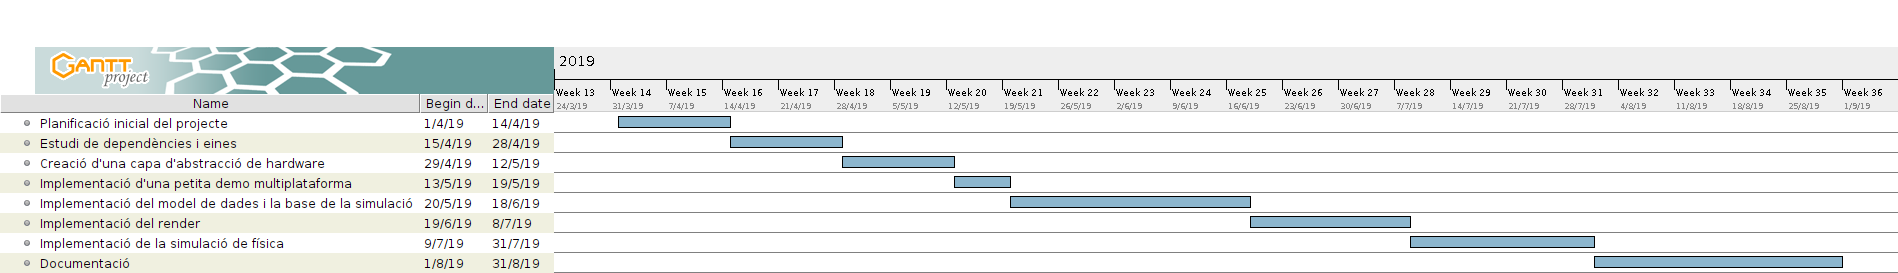
\includegraphics[angle=90,origin=c,scale=0.35]{img/planificacioOG}
  \caption{Diagrama de la planificació original}
\end{figure}
\section{Planificació final}
En la planificació final actual es van afegir diverses tasques que es descriuen a continuació. Cal esmentar que s'ha afegit detall a posteriori a la planificació per oferir una millor explicació.
\begin{itemize}
  \item{Refinament i neteja de bugs: }Fase on netejar bugs i problemes pendents.
  \item{Refactorització i neteja de codi: }Fase per fer canvis no-funcionals al codi per tal de posar-nos al dia amb el deute tècnic. Això inclou simplificacions de codi, millor repartiment del codi en funcions i classes, i possiblement refer des de 0 algunes funcions o classes si és necessari.
  \item{Millores en l'implementació de la física: }Fase on acabar de refinar els càlculs de física. Implementació de co\lgem isions entre nodes i optimització dels càlculs entre entitats.
  \item{Optimitzacions de renderitzat: }Fase d'optimització i neteja del procés de renderitzat per tal d'obtenir un millor rendiment.
  \item{Creació d'uin framework per a interfícies d'usuari: }Fase per crear el framework que facilitarà fer la interfície d'usuari del joc.
  \item{Disseny i implementació d'una interfície senzilla per la demo: }Fase on utilitzarem el framework que hem creat per fer una interfície d'usuari per la demo del joc.
  \item{Implementació d'un sistema per a nodes prefabricats + editor gràfic: }Fase on implementarem un sistema per crear i posar en el joc nodes prefabricats. Un node prefabricat pot ser des d'un vehicle terrestre format per un parell de blocs, a una estació espacial de milers de blocs.
  \item{Implementació d'una màquina d'estats pel jugador: }Fase on implementarem una senzilla màquina d'estas per controlar al jugador (o altres entitats). Això permetrà que el jugador tingui disponibles diferents accions, com per exemple, a l'estar al aire respecte quan està amb els peus a terra.
  \item{Implementació del sistema de propulsió de nodes: }Fase on implementarem un sistema que simularà diversos motors de propulsió juntament amb el combustible. Això inclou la gestió de diversos combustibles, el consum i aprovisionament de combustible, i la generació de forces a partir dels motors.
  \item{Disseny i implementació d'un sistema de blocs interactuables: }Fase on crearem un sistema per permetre la interacció entre entitats i blocs, de forma que una entitat pugui seure en una cadira, o pugui fer accions com obrir portes o controlar màquines.
  \item{Creació de contingut per la demo: }Fase on crearem contingut per la demo, com per exemple generadors de terreny per als planetes, o naus prefabricades que el jugador pugui pilotar.
  \item{Disseny i creació d'un sistema Observer per a esdeveniments del joc: }Fase on implementarem un Observer per poder desacoblar parts del joc que no ho necessitin. Per exemple, enviar esdeveniments a un observador permetria activar una fita quan el jugador fa un salt de més de 100 metres, sense que el sistema de fites i el sistema de física estiguin altament acoblats.
  \item{Implementació de projectils i sistema de salut: }Fase on implementarem un senzill sistema per tal que les entitats puguin disparar projectils, i perdin salut o siguin eliminats al rebre dany d'aquests.
  \item{Refinament final: }Fase per a fer els últims retocs i netejar bugs pendents.
  \item{Documentació: }Fase per finalitzar la documentació del projecte.
\end{itemize}
\begin{figure}[H]
  \centering
  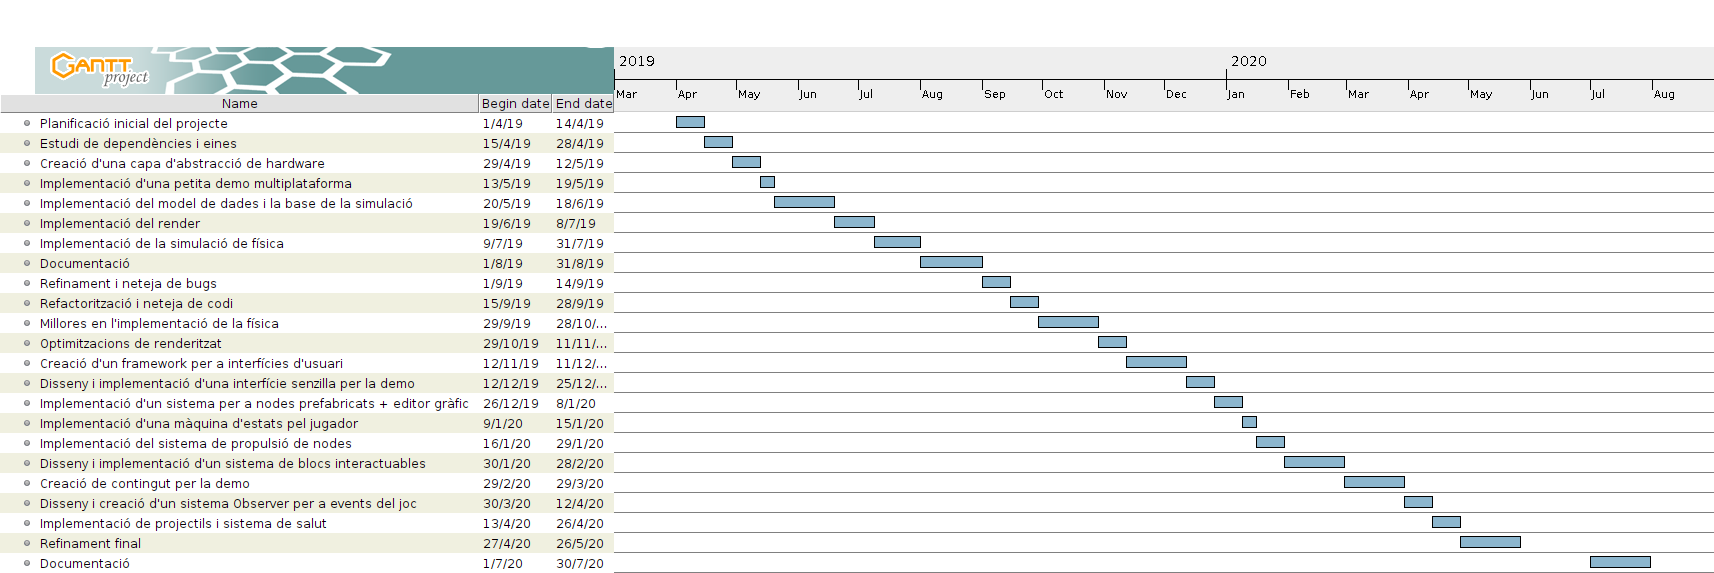
\includegraphics[angle=90,origin=c,scale=0.4]{img/novaPlanificacio}
  \caption{Diagrama de la planificació final}
\end{figure}

